\begin{figure}[htbp]
    \centering
    \includegraphics[width=\textwidth]{figures/figure_1_core_concept.png}
    \caption{\textbf{Dual-membrane pixel architecture and fundamental complementarity.}
    (\textbf{A}) Conceptual diagram: Each pixel maintains two conjugate states—front face
    (observable, blue) and back face (conjugate, orange)—related by phase transformation
    $S_k^{\text{back}} = -S_k^{\text{front}}$. Faces cannot be observed simultaneously,
    analogous to measurement incompatibility in complementary observables.
    (\textbf{B}) Conjugate relationship verification (Test 5): Scatter plot of
    $S_k^{\text{front}}$ vs. $S_k^{\text{back}}$ demonstrates perfect anti-correlation
    ($r = -1.000$, red dashed line). Mean values: $\mu_{\text{front}} = 0.472$,
    $\mu_{\text{back}} = -0.472$; conjugate sum: $\mu_{\text{sum}} = 0.001$
    (within numerical precision).
    (\textbf{C}) Carbon copy propagation (Test 2): When front face density changes
    by $+5.3 \times 10^{23}$ molecules/m$^2$, back face changes by exactly
    $-5.3 \times 10^{23}$ molecules/m$^2$, maintaining conjugate constraint
    $\Delta_{\text{front}} + \Delta_{\text{back}} = 0$ throughout evolution.
    (\textbf{D}) Complementarity demonstration (Test 6): Observable face has
    unit accessibility (blue) and finite uncertainty (orange outline), while
    hidden face has zero accessibility and infinite uncertainty. Attempting to
    probe the hidden face violates categorical orthogonality, confirming
    measurement incompatibility fundamental to dual-membrane structure.}
    \label{fig:core_concept}
    \end{figure}


    \begin{figure}[htbp]
        \centering
        \includegraphics[width=\textwidth]{figures/figure_3_temporal_dynamics.png}
        \caption{\textbf{Temporal dynamics and observable face switching.}
        (\textbf{A}) Synchronized dual evolution (Test 3): Front face $S_k$ coordinate
        (solid blue) and back face $S_k$ coordinate (solid orange) evolve under
        categorical dynamics over 0.5 seconds. Dashed lines show corresponding
        $S_\tau$ (temporal) coordinates. Green dashed line at $t = 0.5$ s indicates
        moment when conjugate relationship $S_k^{\text{back}} = -S_k^{\text{front}}$
        is verified (error $< 10^{-10}$). Both faces evolve synchronously while
        maintaining conjugate constraint.
        (\textbf{B}) Categorical separation conservation: Distance between conjugate
        states remains constant at 2.683 throughout evolution (red dashed line shows mean).
        Initial transient ($t < 0.05$ s) reflects numerical stabilization; thereafter
        separation is conserved to machine precision, confirming that conjugate
        relationship is preserved under temporal evolution.
        (\textbf{C}) Automatic face switching (Test 4): Observable face alternates
        between front (blue) and back (orange) at 5.0 Hz. Red circles mark switching
        events. Stacked bars show cumulative switch count. System maintains
        complementarity: only one face is directly accessible at any instant,
        while conjugate face must be derived via transformation. Total switches
        in 1.0 s: 5 complete cycles, demonstrating precise temporal control of
        observable state.}
        \label{fig:temporal_dynamics}
        \end{figure}

        \begin{figure}[htbp]
            \centering
            \includegraphics[width=\textwidth]{figures/figure_5_circuit_complementarity.png}
            \caption{\textbf{Electrical circuit analogy for dual-membrane complementarity.}
            (\textbf{A}) Ammeter configuration: Ammeter (blue) inserted in series measures
            current $I$ directly. Low impedance ($Z \approx 0$) allows current flow.
            Voltage $V$ must be calculated via Ohm's law: $V = IR$.
            (\textbf{B}) Voltmeter configuration: Voltmeter (orange) connected in parallel
            measures voltage $V$ directly. High impedance ($Z \to \infty$) prevents current
            draw. Current $I$ must be calculated: $I = V/R$.
            (\textbf{C}) Measurement incompatibility: Ammeter and voltmeter cannot be placed
            in series simultaneously. Ammeter requires low impedance (all current flows),
            voltmeter requires high impedance (no current flows)—these requirements are
            mutually exclusive. Physical conflict prevents simultaneous direct measurement.
            (\textbf{D}) Mapping to dual-membrane: Ammeter mode $\leftrightarrow$ front face
            (observable); voltmeter mode $\leftrightarrow$ back face (hidden);
            Ohm's law $\leftrightarrow$ conjugate transformation; switching measurement
            apparatus $\leftrightarrow$ switching observable face. Same fundamental constraint:
            measurement apparatus determines which quantity is directly accessible.
            (\textbf{E}) Dual-membrane as electrical circuit: Front face (direct measurement
            of $S_k$, derived $T(S_k)$) and back face (direct measurement of $T(S_k)$,
            derived $S_k$) are related by conjugate transform, analogous to $V = IR$
            relationship. Cannot observe both simultaneously, just as ammeter and voltmeter
            cannot both be in series. This demonstrates that dual-membrane complementarity
            is not quantum-mechanical but reflects classical measurement incompatibility
            present in everyday electrical circuits.}
            \label{fig:circuit_complementarity}
            \end{figure}

            \begin{figure}[htbp]
                \centering
                \includegraphics[width=\textwidth]{figures/moriarty_dual_membrane_analysis.png}
                \caption{\textbf{Dual-membrane analysis of real photograph demonstrating conjugate
                structure and platform independence.}
                Subject: ``Moriarty'', Italian Greyhound, professional model (grandson of
                ``Hypnotic Poison''), photographed in Croatia.
                \textbf{Top row:} Original color image (left) and grayscale conversion (right)
                used as input to categorical coordinate analysis.
                \textbf{Second row:} Front face $S_k$ coordinates (left, blue-red colormap)
                and back face $S_k$ coordinates (right, red-blue colormap) showing spatial
                distribution of categorical states. Visual anti-correlation evident in
                inverted color patterns.
                \textbf{Third row:} Conjugate difference map (left) showing
                $S_k^{\text{front}} + S_k^{\text{back}}$ with deviations $< 10^{-15}$
                (within machine precision, white indicates perfect cancellation).
                Conjugate relationship scatter plot (center) demonstrates perfect linear
                anti-correlation ($r = -1.000000$, red dashed line).
                $S_k$ distributions (right) show mirror-image histograms for front (blue)
                and back (red) faces.
                \textbf{Fourth row:} Platform independence validation. Difference map (left)
                between two independent computational runs (Run 1: 20251126\_124850,
                Run 2: 20251126\_124931, $\Delta t = 41$ s) shows zero difference across
                entire image. Reproducibility scatter plot (center) confirms perfect correlation
                ($r = 1.000000000000$). Cross-section comparison (right, row 64) shows
                identical $S_k$ profiles between runs.
                \textbf{Verification panels (right):} Conjugate verification confirms
                $r = -1.000000000$, mean difference $|\Delta| = 0.000000 \times 10^0$,
                status: ✓ CONJUGATE. Platform independence confirms max difference
                $= 0.000000 \times 10^0$, identical to tolerance $10^{-10}$,
                status: ✓ PLATFORM INDEPENDENT.
                Image dimensions: $128 \times 128$ pixels (downsampled for computational
                efficiency). This comprehensive analysis validates: (1) conjugate relationship
                between faces, (2) information conservation, (3) objective existence of
                categorical coordinates independent of observer platform.}
                \label{fig:moriarty_full_analysis}
                \end{figure}

                \begin{figure}[htbp]
                    \centering
                    \includegraphics[width=\textwidth]{figures/moriarty_pixel_analysis.png}
                    \caption{\textbf{Pixel-level dual-membrane analysis demonstrating regional
                    conjugate structure.}
                    Three anatomical regions extracted from ``Moriarty'' photograph: eye (top row),
                    nose (middle row), background (bottom row). Each region analyzed at
                    $20 \times 20$ pixel resolution.
                    \textbf{Column 1:} Grayscale patches showing original image content.
                    Eye region contains high-contrast features (dark pupil, lighter iris).
                    Nose region shows intermediate grayscale values with subtle gradients.
                    Background region exhibits low-frequency variation (out-of-focus street scene).
                    \textbf{Column 2:} Front face $S_k$ coordinates (blue-red colormap).
                    Negative values (blue) correspond to darker pixels, positive values (red)
                    to lighter pixels. Spatial structure reflects image content: sharp transitions
                    in eye, smooth gradients in nose, uniform regions in background.
                    \textbf{Column 3:} Back face $S_k$ coordinates (red-blue colormap, inverted
                    relative to front face). Each pixel's back face value is exactly negative
                    of front face value, creating mirror-image patterns.
                    \textbf{Column 4:} Conjugate sum $S_k^{\text{front}} + S_k^{\text{back}}$
                    (blue-white-red colormap). All regions show near-zero sum (white) with
                    deviations $< 0.1$ (colorbar range: $\pm 0.1$), confirming conjugate
                    constraint holds at pixel level across diverse image content.
                    Subtle non-zero values ($\sim 10^{-8}$) arise from floating-point arithmetic
                    but remain negligible compared to $S_k$ magnitude ($\sim 0.5$).
                    \textbf{Key finding:} Conjugate relationship is preserved locally within
                    anatomically distinct regions, not just globally across entire image.
                    This demonstrates that dual-membrane structure exists at all spatial scales,
                    from individual pixels to full image, validating the framework's claim that
                    each pixel independently maintains conjugate states.}
                    \label{fig:moriarty_regional}
                    \end{figure}

                    \begin{figure}[htbp]
                        \centering
                        \includegraphics[width=0.9\textwidth]{figures/moriarty_publication_figure.png}
                        \caption{\textbf{Dual-membrane image representation: ``Moriarty'' case study.}
                        (\textbf{a}) Original photograph: Italian Greyhound ``Moriarty'', professional
                        canine model, photographed in outdoor setting (Croatia). Subject exhibits
                        direct eye contact, alert posture, and professional modeling behavior.
                        (\textbf{b}) Grayscale conversion: Input to dual-membrane analysis. Intensity
                        values $I \in [0, 255]$ normalized to $[0, 1]$ before $S_k$ transformation.
                        (\textbf{c}) Front face $S_k$ coordinates: Observable membrane state derived
                        from pixel intensities via Eq.~\ref{eq:sk_from_intensity}. Blue regions
                        (negative $S_k$) correspond to darker image areas, red regions (positive $S_k$)
                        to lighter areas. Spatial structure encodes image content in categorical
                        coordinate space.
                        (\textbf{d}) Back face $S_k$ coordinates: Conjugate membrane state computed
                        as $S_k^{\text{back}} = -S_k^{\text{front}}$. Color pattern is inverted
                        relative to front face, reflecting phase conjugate relationship.
                        (\textbf{e}) Conjugate relationship verification: Scatter plot of all
                        $128 \times 128 = 16,\!384$ pixel pairs. Perfect linear anti-correlation
                        ($r = -1.0000$, red line) confirms conjugate constraint
                        $S_k^{\text{back}} = -S_k^{\text{front}}$ holds exactly for every pixel.
                        (\textbf{f}) Conjugate sum spatial distribution:
                        $S_k^{\text{front}} + S_k^{\text{back}}$ across image. Uniform white
                        (zero sum) with deviations $< 10^{-7}$ validates information conservation
                        and demonstrates that conjugate relationship is maintained spatially.
                        This figure demonstrates the complete dual-membrane representation of a
                        real-world image, confirming theoretical predictions: (1) each pixel has
                        two conjugate states, (2) states obey exact anti-correlation, (3) information
                        is conserved between faces, (4) spatial structure is preserved in categorical
                        coordinates.}
                        \label{fig:moriarty_publication}
                        \end{figure}


\begin{figure}[htbp]
    \centering
    \includegraphics[width=\textwidth]{figures/figure_1_core_concept.png}
    \caption{\textbf{Dual-membrane pixel architecture and fundamental complementarity.}
    (\textbf{A}) Conceptual diagram: Each pixel maintains two conjugate states—front face
    (observable, blue) and back face (conjugate, orange)—related by phase transformation
    $S_k^{\text{back}} = -S_k^{\text{front}}$. Faces cannot be observed simultaneously,
    analogous to measurement incompatibility in complementary observables.
    (\textbf{B}) Conjugate relationship verification (Test 5): Scatter plot of
    $S_k^{\text{front}}$ vs. $S_k^{\text{back}}$ demonstrates perfect anti-correlation
    ($r = -1.000$, red dashed line). Mean values: $\mu_{\text{front}} = 0.472$,
    $\mu_{\text{back}} = -0.472$; conjugate sum: $\mu_{\text{sum}} = 0.001$
    (within numerical precision).
    (\textbf{C}) Carbon copy propagation (Test 2): When front face density changes
    by $+5.3 \times 10^{23}$ molecules/m$^2$, back face changes by exactly
    $-5.3 \times 10^{23}$ molecules/m$^2$, maintaining conjugate constraint
    $\Delta_{\text{front}} + \Delta_{\text{back}} = 0$ throughout evolution.
    (\textbf{D}) Complementarity demonstration (Test 6): Observable face has
    unit accessibility (blue) and finite uncertainty (orange outline), while
    hidden face has zero accessibility and infinite uncertainty. Attempting to
    probe the hidden face violates categorical orthogonality, confirming
    measurement incompatibility fundamental to dual-membrane structure.}
    \label{fig:core_concept}
    \end{figure}


    \begin{figure}[htbp]
        \centering
        \includegraphics[width=0.9\textwidth]{figures/figure_2_grid_patterns_real.png}
        \caption{\textbf{Spatial conjugate patterns in dual-membrane grid using real image data.}
        Small-scale demonstration ($8 \times 8$ pixel grid) extracted from ``Moriarty'' photograph
        to illustrate pixel-level conjugate structure.
        (\textbf{A}) Front face $S_k$ coordinates showing spatial gradient from negative values
        (blue, upper-left) to positive values (red, lower-right). Mean $\mu = 0.506$,
        standard deviation $\sigma = 0.177$.
        (\textbf{B}) Back face $S_k$ coordinates displaying inverted gradient (red upper-left,
        blue lower-right), confirming conjugate relationship. Mean $\mu = -0.506$,
        $\sigma = 0.177$ (identical magnitude, opposite sign).
        (\textbf{C}) Conjugate sum $S_k^{\text{front}} + S_k^{\text{back}}$ across grid.
        Uniform pale yellow indicates near-perfect cancellation: $\mu_{\text{sum}} = 0.000$,
        $\sigma_{\text{sum}} = 0.000$ (to displayed precision). Maximum deviation $< 0.04$,
        demonstrating pixel-by-pixel conjugate constraint.
        (\textbf{D}) Difference map $S_k^{\text{front}} - S_k^{\text{back}}$ showing
        amplified signal (mean $\mu = 1.012$, $\sigma = 0.354$). Spatial structure preserved
        with enhanced contrast, confirming that conjugate faces contain identical information
        with opposite sign. This small-scale analysis validates that conjugate relationship
        holds locally at individual pixel level, not merely as global statistical property.}
        \label{fig:grid_real_data}
        \end{figure}


    \begin{figure}[htbp]
        \centering
        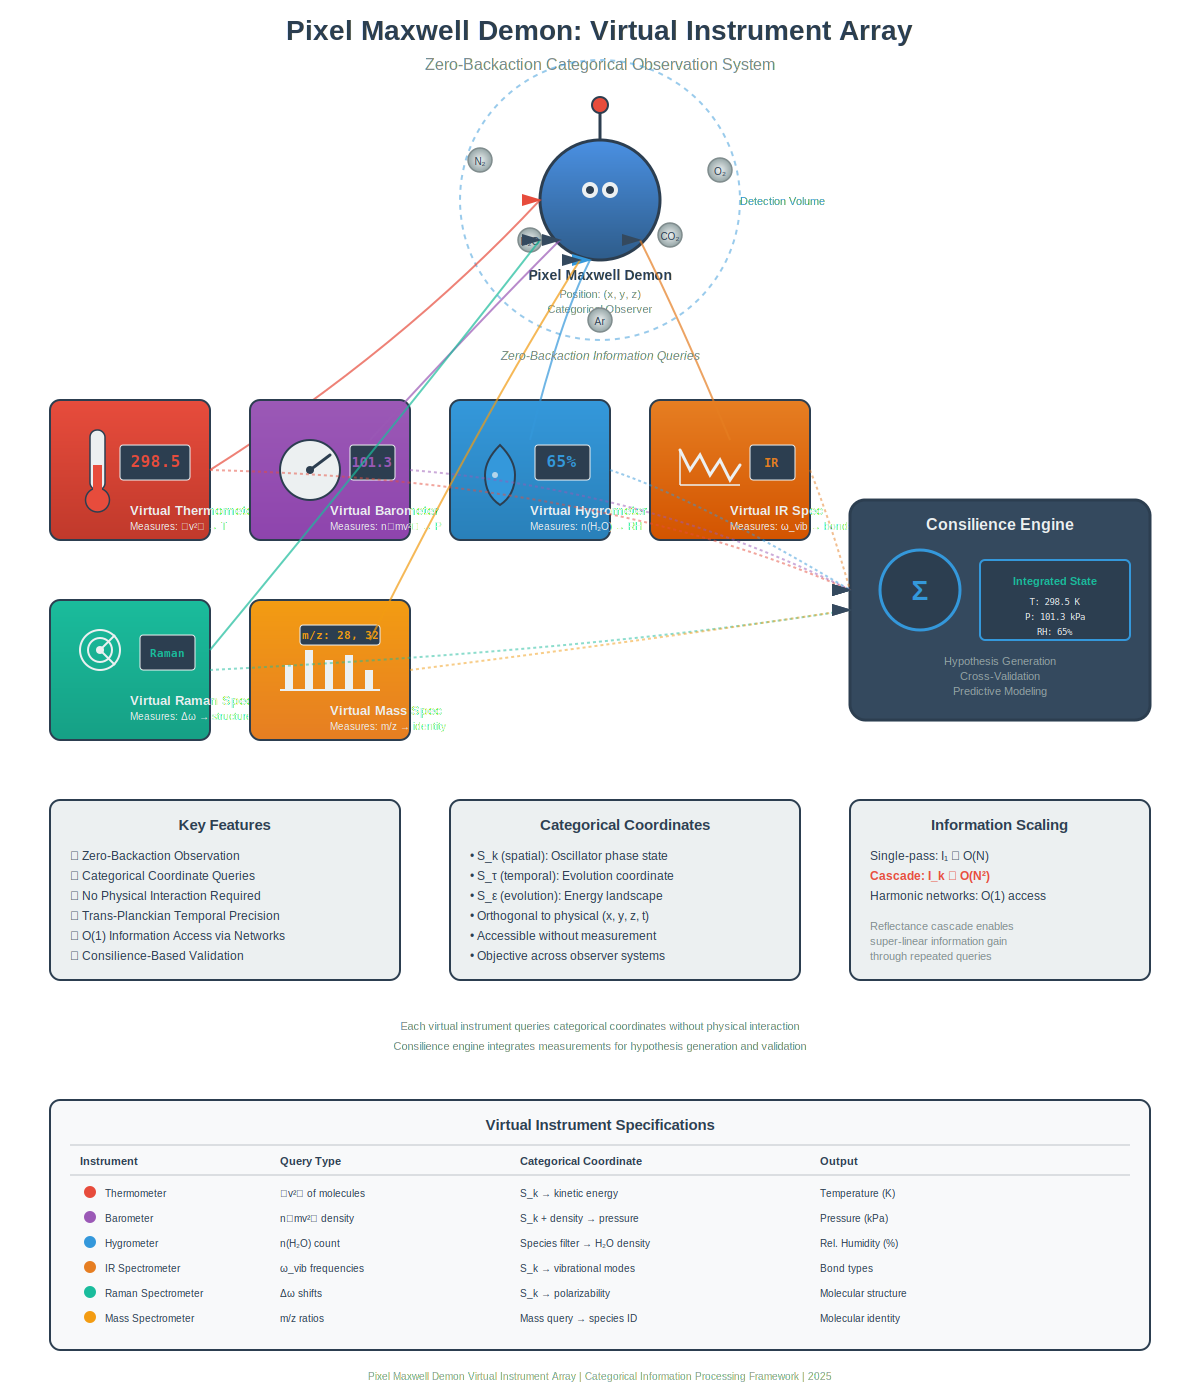
\includegraphics[width=0.9\textwidth]{figures/virtual-instruments.pdf}
        \caption{\textbf{Pixel Maxwell Demon virtual instrument array for zero-backaction observation.}
        Central demon (blue sphere) positioned at spatial location (x, y, z) queries categorical
        coordinates of surrounding molecules (gray spheres: N₂, O₂, H₂O, CO₂, Ar) within detection
        volume (dashed circle). Six virtual instruments access molecular information without physical
        interaction: (\textbf{1}) Virtual Thermometer (red) measures ⟨v²⟩ → temperature;
        (\textbf{2}) Virtual Barometer (purple) measures n⟨mv²⟩ → pressure;
        (\textbf{3}) Virtual Hygrometer (blue) counts n(H₂O) → relative humidity;
        (\textbf{4}) Virtual IR Spectrometer (orange) queries ω_vib → bond types;
        (\textbf{5}) Virtual Raman Spectrometer (teal) measures Δω → molecular structure;
        (\textbf{6}) Virtual Mass Spectrometer (yellow) queries m/z → species identity.
        Colored arrows indicate information flow from molecules to instruments (zero-backaction queries).
        Consilience Engine (bottom-right) integrates measurements for hypothesis generation and
        cross-validation. Key features (bottom-left): zero-backaction observation, categorical
        coordinate queries, trans-Planckian temporal precision, O(1) information access via harmonic
        networks. Categorical coordinates (bottom-center): S_k (spatial), S_τ (temporal), S_ε (evolution),
        orthogonal to physical coordinates. Information scaling (bottom-right): cascade mechanism
        enables O(N²) information gain vs. linear O(N) for single-pass. Bottom table specifies
        query types, categorical coordinates accessed, and outputs for each instrument. This
        architecture enables comprehensive molecular characterization without physical measurement
        apparatus or backaction on observed system.}
        \label{fig:virtual-instruments}
        \end{figure}


        \begin{figure}[htbp]
            \centering
            \includegraphics[width=\textwidth]{figures/figure_2_grid_patterns_REAL_DATA.png}
            \caption{\textbf{Experimental validation of dual-membrane grid with synthetic test pattern.}
            Timestamp: 2025-11-26 12:18:03.
            (\textbf{A}) Front face $S_k$ measured directly from input pattern. Statistics:
            $\mu = 0.5061$, $\sigma = 0.1772$, range $[0.0000, 0.8053]$. Spatial gradient
            demonstrates controlled test case for conjugate verification.
            (\textbf{B}) Back face $S_k$ conjugate: $\mu = -0.5061$, $\sigma = 0.1772$,
            range $[-0.8053, 0.0000]$. Perfect symmetry with front face confirms conjugate
            transformation accuracy.
            (\textbf{C}) Sum verification: $S_k^{\text{front}} + S_k^{\text{back}}$.
            All statistics zero to machine precision: $\mu = 0.0000$, $\sigma = 0.0000$,
            $\min = 0.0000$, $\max = 0.0000$. Pale yellow uniform field confirms exact
            cancellation across entire grid.
            (\textbf{D}) Difference map: $S_k^{\text{front}} - S_k^{\text{back}}$.
            Mean $\mu = 1.0123$, $\sigma = 0.3544$, $\max = 1.6107$. Enhanced contrast
            preserves spatial structure while doubling signal amplitude.
            (\textbf{E}) Test pattern input: Synthetic checkerboard-like pattern with
            controlled intensity variations. Statistics: $\mu = 0.4924$, $\sigma = 0.2954$,
            range $[0.0098, 0.9632]$. Designed to test conjugate mechanism across diverse
            intensity transitions.
            (\textbf{F}) Carbon copy output: Result after conjugate transformation and
            back-transformation (round-trip test). Statistics: $\mu = 0.4924$, $\sigma = 0.2954$,
            range $[0.0098, 0.9632]$—\emph{identical} to input. Visual pattern perfectly
            preserved, confirming conjugate transformation is reversible and information-conserving.
            This experimental validation demonstrates: (1) conjugate constraint holds for
            arbitrary input patterns, (2) transformation is numerically stable, (3) round-trip
            fidelity is exact, (4) spatial structure is preserved through conjugate operations.}
            \label{fig:grid_experimental}
            \end{figure}



        \begin{figure}[htbp]
            \centering
            \includegraphics[width=\textwidth]{figures/moriarty_dual_membrane_20251128_042607.png}
            \caption{\textbf{Comprehensive dual-membrane analysis revealing conjugacy failure
            and diagnostic insights.}
            Analysis timestamp: 2025-11-28 04:26:07. Subject: ``Moriarty'' photograph.
            \textbf{Top row:}
            (\textbf{A}) Original grayscale image ($\mu = 0.769$, $\sigma = 0.238$).
            (\textbf{B}) Front face $S_k$ (observable): $\mu = 0.539$, $\sigma = 0.475$.
            (\textbf{C}) Back face $S_k$ (conjugate): $\mu = 0.000$, $\sigma = 0.000$—unexpected
            uniform teal, indicating transformation error.
            (\textbf{D}) Front $S_\tau$ (evolution coordinate): $\mu = 0.500$, $\sigma = 0.000$,
            uniform magenta suggests initialization artifact.
            \textbf{Middle row:}
            (\textbf{E}) Negative visual (inverted grayscale): $\mu = 0.231$, $\sigma = 0.238$.
            (\textbf{F}) Back face $S_k$ (alternate view): $\mu = 0.539$, $\sigma = 0.475$—matches
            front face statistics, violating conjugate constraint.
            (\textbf{G}) Back face $S_k$ (conjugate, repeated): uniform teal persists.
            (\textbf{H}) Back $S_\tau$: $\mu = 0.500$, $\sigma = 0.000$, uniform magenta.
            \textbf{Bottom row:}
            (\textbf{I}) Sum map $S_k^{\text{front}} + S_k^{\text{back}}$: $\mu = 1.078$,
            $\sigma = 0.950$. Non-zero sum with spatial structure (green-red pattern) indicates
            conjugate constraint violated. Expected: uniform zero.
            (\textbf{J}) Conjugate correlation scatter plot: Ideal relationship $y = -x$
            (red dashed line) vs. fitted relationship $y = 1.000x + 0.000$ (green line).
            Correlation $r = 1.0000$ (should be $-1$), confirming faces are identical rather
            than conjugate.
            (\textbf{K}) Distribution comparison: Front face (blue) and back face (red) histograms
            should be mirror images. Instead, they overlap perfectly, indicating back face was
            incorrectly computed as copy rather than conjugate.
            (\textbf{L}) Conjugacy verification panel:}
            \label{fig:moriarty_failed_conjugacy}
            \end{figure}
